\documentclass[a4paper,10pt]{article}

\usepackage[utf8]{inputenc}
\usepackage[T1]{fontenc}
\usepackage{graphicx}
\usepackage{listings}
\usepackage[english]{babel}
\usepackage{tabularx}
\usepackage{tikz}
\usepackage{enumitem}

\title{Linux Desktop Security}
\author{Maximilian Heim}




\begin{document}

\maketitle
\thispagestyle{empty}
\newpage
\tableofcontents
\thispagestyle{empty}
\newpage
\setcounter{page}{1}
\section{Introduction}
Welcome to the Linux Desktop Security tutorial! In this tutorial we will show how to set up a Linux desktop system from scratch at the example of Ubuntu. This tutorial is aimed at anyone that wants to harden their setup, from beginner to advanced it will guide you from the very beginning in an Ubuntu installation step by step so even people that are new to Linux distributions can follow easily. It is important to note that this tutorial is for Ubuntu Desktop, while most things also apply to Ubuntu Server, you need to perform additional measures to harden an Ubuntu/Linux server.

\vspace{5mm}

\begin{center}

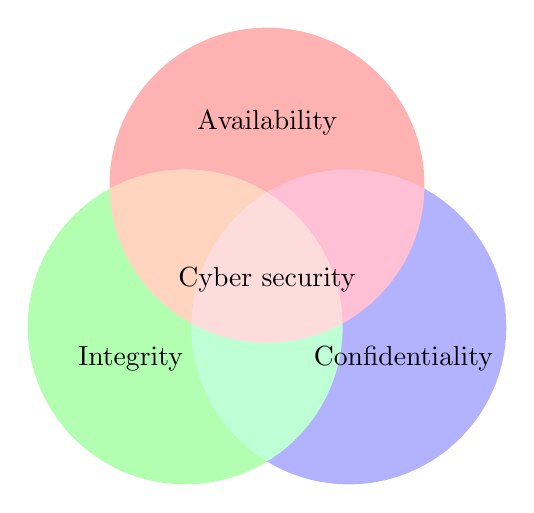
\begin{tikzpicture}
\begin{scope}[blend group=soft light]
\fill[red!30!white](90:1.2) circle (2);
\fill[green!30!white](210:1.2) circle (2);
\fill[blue!30!white](330:1.2) circle (2);

\end{scope}

\node at (90:2) {Availability};
\node at (210:2) {Integrity};
\node at (330:2) {Confidentiality};
\node {Cyber security};
\end{tikzpicture}

\end{center}

\begin{center}
The three goals in cyber security
\end{center}

\vspace{5mm}

\section{Ubuntu}

\paragraph{GNU/Linux}
GNU/Linux, usually just referred to as Linux are Unix like, free and open source operating systems which base on the Linux kernel. There are hundreds of distributions of Linux, each distribution has a set of GNU software pre-installed. It has a modular design featuring high customizability.

\paragraph{Ubuntu}
Ubuntu or Ubuntu Linux is a Linux distribution developed by Canonical, based on Debian. It was first released at October 20th 2004 and since then its popularity steadily rose. Ubuntu updates are released in a 6 Month cycle with regular minor updates. Every 2 Years Canonical releases a long-term support release which has a maintenance period of 5 Years.

\paragraph{For who is Ubuntu?}

Ubuntu is for anyone. It is a relatively simple Linux distribution which fits the needs of simple desktop user to professionals.

\paragraph{Why Ubuntu?}
The question should rather be Why Linux?. Linux distributions are highly customizable operating systems with alterable look via the desktop environments and package systems. In addition to that Linux distributions have a safer design as Windows.

\section{Setting up Ubuntu}
\subsection{Creating a bootable drive}

\begin{itemize}[leftmargin=*]
\item In order to install Ubuntu, the first thing you have to do is either buy an Ubuntu disk copy or create a bootable disk or USB drive. This is where the data necessary for the Ubuntu installation is stored on.
\item For creating the bootable drive, the first thing you have to is downloading the newest version of Ubuntu Desktop from www.ubuntu.com/download\\/desktop
\item After that you need to download a software which is able to create bootable disk/USB drives. For USB drives the open source software Rufus is highly recommendable.
\item Now you need to plug in the USB stick into your computer and if you have any data stored on the USB stick you need to save your files because the tool will format your USB drive, deleting all data stored on it. 
\item The next step is opening the tool and selecting the USB stick you wanna use, after that select the Ubuntu iso file from your storage.
\item The rest is fine if you leave it on default. It should look similar to this.

\end{itemize}
\begin{center}
\includegraphics[scale=0.5]{Rufus ubuntu}
\end{center}
\begin{itemize}[leftmargin=*]

\item Next thing you want to do is press start and the tool will start to write the data onto the USB stick. If this is done you can unplug the USB stick.
\end{itemize}


\subsection{Installing Ubuntu onto the system}
\begin{itemize}[leftmargin=*]
\item Now you can go to the computer you want to install Ubuntu onto.
\item Plug the USB stick into the computer and turn it on. Directly at the start of the computer there will usually be an UEFI/BIOS screen and it will display some hotkeys, here you should press the hotkey which opens the boot menu.
\item When you are in the boot menu you should select the USB stick and boot from it.
\item When everything went clean you should get a screen which lets you select a language for the installation and on the right side "Install Ubuntu", now you should click that button which will lead you to the first step of the setup which is the keyboard layout, here you need to select the keyboard layout, there is also an automatic detection for that. If you're done with that you can proceed to the next step. 
\item This will let you decide if you want the "normal" Ubuntu installation or the minimal one. The minimal installation is the safer one because it installs less programs but you have to download some software later on, it is recommended to use the minimal installation but in case you want to go with the standard set up you can do that, we will later explain which programs to remove. Here you should also make sure the "Download updates while installing" option is activated. If you're done with that you can proceed to the next step.
\item Here you can decide if you want to erase the complete hard drive and make a clean installation or you can select a partition to install on if you want to set up a dual boot computer. If you chose the erase disk option you can also activate LVM and encrypt the disk which provides additional safety from data theft.
\item Now you need to select your time zone. After that comes the last step which is setting up an user account.
\item The important part about this is choosing a safe password, meaning that you shouldn't use words which are related to you or people you know, should have roughly 12 characters, a mix of capitalized and non capitalized letters, numbers and special characters is perfect. Make sure the checkbox "require password to log in" is checked.
\item After continuing Ubuntu will take some time to set everything up and after that you have to restart the system. Now you have to setup a few more things.
\item After the restart Ubuntu will display a window which will allow you to setup Canonial Live Patch, this is highly recommended as it is able to apply kernel patches without restarting, increasing security.\cite{ubuntucanoniallivepatch} 
\item The next thing you have to do is decide whether or not you want to send anonymous user statistics to the Ubuntu developers, this isn't a security threat because it contains no personal information, you can leave it on as it lets the Ubuntu developers know what to focus on.
\item The next screen will ask if you want to use location services, usually you can just leave it deactivated as you don't really need it.
\item Now Ubuntu will display the Ubuntu Software program which easily lets you download programs which you might want, but you should wait before you do that because we have to modify the software which can be downloaded via this Software Center.
\item After that Ubuntu may or may not tell you that an update is available. You should install this.
\item Now the basic setup is complete and we can continue with configuring the more specific things.
\end{itemize}



\subsection{Uninstalling unneeded software}

\paragraph{Introduction}
Unneeded software represents a security threat because software has vulnerabilities, so you should always uninstall anything you don't need anymore. If you chose the minimal installation you can leave everything as it is but if you've chosen the standard installation you might need to remove a few programs and packages.


\subsubsection{Default programs}

\paragraph{Remove unneeded programs}

\begin{itemize}[leftmargin=*]
\item First you have to open the Ubuntu Software program, here you have to switch to the tab Installed which will display currently installed software. 
\item We will provide a list of items which are recommended to remove, you can keep some if you think you need them but its highly recommended to remove them.

\item AisleRiot Solitaire, Cheese, GNOME Mahjong, GNOME Mines, GNOME Sudoku, Remmina, Rythmbox.
\end{itemize}





\subsection{Removing untrusted publishers}
\paragraph{Introduction}
Not every published software should necessarily be trusted, in order to make sure you only install clean software you have to configure specific settings.
\paragraph{Configuration}
\begin{itemize}[leftmargin=*]
\item Now you have to open the Software \& Updates program via the Show Applications button in the bottom left corner of your screen. 
\item Once in there and in the Ubuntu Software tab you should remove the ticks for restricted and multiverse packages.  
\item In the Other Software tab you should remove the tick for the Canonical Partners packages. In the tab Updates you should remove the tick for Unsupported updates. 
\item Now you can close this window and Ubuntu will probably display you a window which tells you the informations about software are out-of-date, you should press the reload button here. 
\item After that you should open the Terminal and run these two commands
\end{itemize}

\begin{center}
\begin{tabular}{c}
\begin{lstlisting}
sudo apt update
\end{lstlisting}
\end{tabular}
\end{center}

\begin{center}
\begin{tabular}{c}
\begin{lstlisting}
sudo apt dist-upgrade
\end{lstlisting}
\end{tabular}
\end{center}

\begin{itemize}[leftmargin=*]
\item now everything is configured and we can proceed to the next step.
\end{itemize}

\subsection{Configuring updates}
\paragraph{Introduction}
Software updates are very important and should be installed as soon as possible, not only do they provide functionality but they often also fix security vulnerabilities which attackers can use to compromise your system. Because of that you should make sure you set up your update settings correctly.

\paragraph{Software \& Updates}
Ubuntu has a pre installed program which helps with managing updates. It is called Software \& Updates and can be found within the Show Applications tab.



\subsection{Permissions}
\paragraph{Introduction}
Permissions are an important part when it comes to security, they decide which entities have access to which parts of a system, if the permissions are set up correctly it can prevent many kinds of attacks and malfunctioning. In the following we will show how permissions work and what to keep in mind when setting them up.


\paragraph{How permissions work}

Linux has a strict hierarchic permission system for it's files, folders and devices. The permission system has 3 different groups of users. There is the group user, which is basically just the owner of the file which by default is the creator of the file, but it can also be set with a command, then there is the group group, which is the owner group of this file which can be set, and lastly there is the group others which is anyone else. Each group has three different permissions, there is the read, write and execute permission. The representation of this is a concatenation of these three groups with the permissions in each of them which looks like this rwxrwxrwx. If a permission isn't given there is a hyphen instead of the letter.
\paragraph{Usage}

\begin{itemize}[leftmargin=*]
\item In order to show the permissions for the elements of a folder you can use the following command
\end{itemize}

\begin{center}
\begin{tabular}{c}
\begin{lstlisting}
ls -al
\end{lstlisting}
\end{tabular}
\end{center}

\begin{itemize}[leftmargin=*]
\item this will display the content of a folder, the -l option will show the long version with information about permissions and size and the -a option also displays hidden items, the folder itself and the super folder. \item In order to change the permissions of an element, you can use the following command
\end{itemize}

\begin{center}
\begin{tabular}{c}
\begin{lstlisting}
chmod <userperm><groupperm><othersperm> <element>
\end{lstlisting}
\end{tabular}
\end{center}

\begin{itemize}[leftmargin=*]
\item the fastest way to do this is using the octal representation of permissions. 
\item For that you have to add the corresponding numbers to the permissions you want to give, 4 is the read permission, 2 is write and 1 is execute, so as example if you want to give user read and write and the group read and the others no permissions you have to use 640. 
\item Additionally you can change the group of an element with the following command
\end{itemize}

\begin{center}
\begin{tabular}{c}
\begin{lstlisting}
chgrp <group> <element>
\end{lstlisting}
\end{tabular}
\end{center}


\begin{itemize}[leftmargin=*]
\item it's important to note that you have to be the owner or superuser of an element to perform this command and that you have to be part of the group you want to change to.
\item Additionally you can also change the owner of the file with the following command
\end{itemize}


\begin{center}
\begin{tabular}{c}
\begin{lstlisting}
chown <user> <element>
\end{lstlisting}
\end{tabular}
\end{center}


\paragraph{Setting up permissions}
\begin{itemize}[leftmargin=*]
\item In information security, the principle of least privilege is a core rule. 
\item The same thing applies to Linux. Users and programs should always have the least privileges/permissions to work properly. It's not necessary to give something more rights as it needs. 
\item In order to decide which permissions something should have the intended use of a system and what parts of the system are used for what are crucial.
\item If you're running a multi user setup at home with people you trust you can just leave most permissions as they are. The owner of the user folder has all permissions and the group and others have read and execute permissions. If you want to exclude people from being able you can change the permission of your user folder to 760 and add the people you trust to the group. 
\item If you're running a multi user set up at work with different people working on different stuff, and you don't want everyone to be able to access everything the same thing applies, you can change the user folders permissions to 770 which allows the owner and the group to access and modify the content, but everyone else alias the others have no permissions.
\end{itemize}

\subsection{Firewall}

\subsubsection{UFW}
\paragraph{Setting up UFW}

\begin{itemize}[leftmargin=*]
\item The next thing you should do is setting up your firewall properly, for that you have to open up your Terminal and type in
\end{itemize}

\begin{center}
\begin{tabular}{c}
\begin{lstlisting}
sudo apt install ufw
\end{lstlisting}
\end{tabular}
\end{center}

\begin{itemize}[leftmargin=*]
\item this will install ufw, that acronym stands for Uncomplicated Firewall, and that is exactly what it is.
\item After that you should make sure it is activated. For that you should use the following command
\end{itemize}

\begin{center}
\begin{tabular}{c}
\begin{lstlisting}
sudo ufw enable
\end{lstlisting}
\end{tabular}
\end{center}


\paragraph{Setting up GUFW}

\begin{itemize}[leftmargin=*]
\item Additionally you can install the gui front-end, it doesn't provide any extra functionality but for users that dislike navigating via console this is a neat feature.
\item You can install it via the following command
\end{itemize}

\begin{center}
\begin{tabular}{c}
\begin{lstlisting}
sudo apt install gufw
\end{lstlisting}
\end{tabular}
\end{center}

\begin{itemize}[leftmargin=*]
\item after the installation you can open it via the following command
\end{itemize}

\begin{center}
\begin{tabular}{c}
\begin{lstlisting}
gufw
\end{lstlisting}
\end{tabular}
\end{center}



\begin{itemize}[leftmargin=*]
\item you may want to check if everything is set up correctly. It should be activated, Incoming should be Denied and Outgoing Allowed.
\end{itemize}


\subsection{Browser}
\subsubsection{Firefox}
\paragraph{Introduction}
It is well known that Firefox is one of the safest browsers out there.\cite{firefoxSafe} Yet it is highly customizable and comes preinstalled with Ubuntu. In the following we will show some useful add-ons for Firefox to improve your privacy and make browsing more enjoyable.

\paragraph{Privacy Badger}
\begin{itemize}[leftmargin=*]
\item Privacy Badger is an add-on for Firefox, developed by EFF Technologists. It stops advertisers and third parties from tracking your internet usage.
\item It doesn't interfere with your browser usage so it's highly recommended to install it. You can install it via the Firefox Add-On webpage.
\item The URL is https://addons.mozilla.org
\end{itemize}

\paragraph{HTTPS Everywhere}
\begin{itemize}[leftmargin=*]
\item HTTPS Everywhere is an add-on for Firefox, developed by EFF Technologists. It encrypts your communications with many websites which will make browsing more secure.
\item It is highly recommended to download this add-on.
\item It may not work on some websites but you can whitelist these in case this happens.
\item The URL is https://addons.mozilla.org
\end{itemize}

\paragraph{DuckDuckGo}
\begin{itemize}[leftmargin=*]
\item DuckDuckGo is an open source add-on for Firefox, developed by Duck Duck Go Inc.. It blocks trackers and changes your default search engine to the DuckDuckGo engine, which values the privacy of their users - in contrast to Google. 
\item It is highly recommended to install this add-on.
\item The URL is https://addons.mozilla.org
\end{itemize}


\subsection{Anti malware software}
\subsubsection*{Introduction}
There is a controversy about whether or not Linux operating systems need anti malware software. This controversy has its root in the fact that 1. Linux distributions have better security system as Windows and 2. For Desktop users Linux is less popular as Windows, making it less beneficial for cyber criminals to spread malware on Linux. But that is only half of the truth, malware infections are still possible, and as we focus on safety in this article we will still recommend using an anti malware software on your Linux system.\cite{mircolanglinuxav} It's always better to be safe than sorry. In the following we will show how to set up two different anti malware softwares. One of them is ClamAV which is a free and open source solution. On the other hand there is Eset NOD32 which is a commercial solution, it's price is roughly 30 € / Year and provides a very good detection rate.




\subsubsection{ClamAV}

\paragraph{Base installation and usage}
\begin{itemize}[leftmargin=*]
\item ClamAV is a free open source anti malware solution for Linux systems.
\item In order to install it on Ubuntu you have to open up your Terminal and execute the following command
\end{itemize}

\begin{center}
\begin{tabular}{c}
\begin{lstlisting}
sudo apt install clamav
\end{lstlisting}
\end{tabular}
\end{center}

\begin{itemize}[leftmargin=*]
\item which will install both clamav and clamav-freshclam, clamav is the actual software and freshclam is used to update the malware signatures.
\end{itemize}
\paragraph{Usage}

\begin{itemize}[leftmargin=*]
\item In order to use the ClamAV you need to open the Ubuntu Terminal and use the command
\end{itemize}

\begin{center}
\begin{tabular}{c}
\begin{lstlisting}
clamscan <File/Directory>
\end{lstlisting}
\end{tabular}
\end{center}


\begin{itemize}[leftmargin=*]
\item you can also not specify any file/directory, this will scan the whole directory.
\item If you have to scan directories which are outside of your user folder you have to add sudo to the command.
\item It is recommended to scan files after you downloaded something from the internet or got an USB stick/hard drive from someone and plan on using it.
\item Also you should scan your complete system once in a while.
\end{itemize}


\paragraph{ClamAV Daemon installation and usage}

\begin{itemize}[leftmargin=*]
\item Additionally to the basic ClamAV program you can install the ClamAV Daemon which is a background service which actively scans your computer for malware.
\item To install it, use the following command
\end{itemize}

\begin{center}
\begin{tabular}{c}
\begin{lstlisting}
sudo apt install clamav-daemon
\end{lstlisting}
\end{tabular}
\end{center}

\begin{itemize}[leftmargin=*]
\item this doesn't require any further modifications and can be left like this.
\end{itemize}

\paragraph{ClamTK installation and usage}

\begin{itemize}[leftmargin=*]
\item Additionally to the basic ClamAV program you can install the ClamTK frontend which is a graphical user interface for ClamAV.
\item In order to install it you can use the following command
\end{itemize}

\begin{center}
\begin{tabular}{c}
\begin{lstlisting}
sudo apt install clamtk
\end{lstlisting}
\end{tabular}
\end{center}

\begin{itemize}[leftmargin=*]
\item the usage is pretty self explanatory and it provides just as much functionality as ClamAV provides as it is just the frontend for it.
\end{itemize}

\subsubsection{Chkrootkit}

\paragraph{Installation}

\begin{itemize}[leftmargin=*]
\item In order to install chkrootkit onto your system you have to use the following command
\end{itemize}

\begin{center}
\begin{tabular}{c}
\begin{lstlisting}
sudo apt install chkrootkit
\end{lstlisting}
\end{tabular}
\end{center}

\paragraph{Usage}
\begin{itemize}[leftmargin=*]
\item In order to use the program you have to use the following command
\end{itemize}

\begin{center}
\begin{tabular}{c}
\begin{lstlisting}
sudo chkrootkit
\end{lstlisting}
\end{tabular}
\end{center}


\begin{itemize}[leftmargin=*]
\item which will scan your computer for root kits. 
\item It is recommended to use this command once in a while to make sure your computer isn't infected.
\end{itemize}


\subsubsection{NOD32}
\paragraph{Installation}

\begin{itemize}[leftmargin=*]
\item First thing you have to do is buy a license for Eset NOD32 on Eset's website and download the software.
\item The next step is right clicking the file and opening the properties, then you have to open the Permissions tab and check the Allow executing file as program checkbox.
\item Before you can open the file you still need to install a package, for that you have to run these three commands in the following order
\end{itemize}

\begin{center}
\begin{tabular}{c}
\begin{lstlisting}
sudo apt-get update

\end{lstlisting}
\end{tabular}
\end{center}

\begin{center}
\begin{tabular}{c}
\begin{lstlisting}
sudo apt-get upgrade
\end{lstlisting}
\end{tabular}
\end{center}

\begin{center}
\begin{tabular}{c}
\begin{lstlisting}
sudo apt-get install libc6:i386
\end{lstlisting}
\end{tabular}
\end{center}

\begin{itemize}[leftmargin=*]
\item when this is done you can start the installer for Eset NOD32, this is a pretty straightforward installation so this won't be described further here.
\item After the installation you need to restart the system for the changes to get active.
\item After the restart the program will start automatically and you have to log in with your account in order to activate the program.
\end{itemize}

\paragraph*{Usage}
\begin{itemize}[leftmargin=*]
\item To scan your system you have to start ESET NOD32 and open the Computer scan tab, here you can chose between different scan types and customize them.
\item It is recommended to do a full scan every once in a while.
\end{itemize}

\subsection{Program isolation}
\paragraph{Introduction}
Ideally you want to run programs with specific permissions so they really only can modify and access what they should modify and access. Alternatively you can run programs in a sandbox. There are several options to achieve this goal, the most popular ones are AppArmor, SeLinux and Firejail, even though AppArmor and SELinux work differently as FireJail they have the same goal, to prevent damage by software. AppArmor is included in Ubuntu by default, hence we will show how to set up Firejail parallel to AppArmor.

\subsubsection{Firejail}
\paragraph{Introduction}
Firejail is a program which reduces the risk of security breaches. It technically isolates a program from the rest of a system by executing programs in a sandbox. By that it can reduce the risk of damaging the system by using exploits or just plain dysfunction. It has more as 350 predefined configurations for commonly used programs and it is beginner friendly. From the aspect of what the application is supposed to do it is very similar to AppArmor which is preinstalled on Ubuntu, even though these two programs use rather different approaches.

\paragraph{Installation}

\begin{itemize}[leftmargin=*]
\item In order to install Firejail you have to open up the Terminal and type in the following commands.
\end{itemize}

\begin{center}
\begin{tabular}{c}
\begin{lstlisting}
sudo apt install firejail
\end{lstlisting}
\end{tabular}
\end{center}

\begin{center}
\begin{tabular}{c}
\begin{lstlisting}
sudo apt install firejail-profiles
\end{lstlisting}
\end{tabular}
\end{center}

\begin{itemize}[leftmargin=*]
\item In addition to the basic installation you can set up the frontend GUI for Firejail alias Firetools.
\item You can install Firetools via the following command

\begin{center}
\begin{tabular}{c}
\begin{lstlisting}
sudo apt install firetools
\end{lstlisting}
\end{tabular}
\end{center}


\end{itemize}




\paragraph{Usage}

\subparagraph{Creating config files}


\subparagraph{Usage via console}

\begin{itemize}[leftmargin=*]
\item The usage of FireJail is pretty straightforward. In order to start a program in a sandbox you have to use the following command
\end{itemize}

\begin{center}
\begin{tabular}{c}
\begin{lstlisting}
firejail <program>
\end{lstlisting}
\end{tabular}
\end{center}

\begin{itemize}[leftmargin=*]
\item where program is the command to open the program you want to run, e.g. firefox, vlc etc..
\item Firejail will first seek a configuration file in the ~/.config/firejail directory and after that in the /etc/firejail directory.
\end{itemize}

\subparagraph{Automatically running programs in Firejail}

\begin{itemize}[leftmargin=*]
\item Alternatively you can create a symbolic link in the /usr/local/bin path that redirects to the Firejail binarie file, this way programs will always be executed in a sandbox environment, regardless of the way they got started.
\item The tool firecfg which is included in the Firejail package supports the user with this configuration and performs this task for every program with an existic FireJail profile. In order to do this you have to use the following command


\end{itemize}




\subsection{VPN}
\paragraph{Introduction}
VPN Stands for Virtual Privet Network is extending a private network onto a public network. A VPN hides your ip and features encrypted connection to the VPN provider you are using. In the following we will show how to set up ExpressVPN

\subsubsection{ExpressVPN}
\paragraph{Introduction}
ExpressVPN is a VPN provider with a very good reputation when it comes to privacy, speed and customer support. It comes with a price which is proportional to these qualities but it is really worth that.

\paragraph{Installation}
\begin{itemize}[leftmargin=*]
\item In order to install ExpressVPN you have to visit the ExpressVPN website which you can find under this link www.expressvpn.com. 
\item First you should setup an account, after that you should log in into your account and buy a licence, it lets you choose from three different plans, pick one which fits ur needs.
\item Then you have to enter your E-Mail adress and choose a payment method.
\item After paying you have to copy the Activation code which gets displayed to you and download the Linux installer.
\item Then you have to install the software via the installer. Once that is done you can open the software and click Set Up ExpressVPN.
\item After that you have to paste the activation code and click Sign In.
\end{itemize}

\paragraph{Usage}
\begin{itemize}[leftmargin=*]
\item The usage of ExpressVPN is pretty straightforward, you can select a server and click the click to connect button to conntect to this server.
\item Now your internet usage is pseudo anonymous and encrypted which will improve your privacy 
\end{itemize}




\subsection{Backups}

\paragraph{Introduction}
As you probably have valuable data you want to make sure is safe, it is highly recommended to create backups of your data every now and then. For that you have several methods like using CD/DVD's, USB, external hard drives and internet. I recommend using USB or a hard drives as they provide much storage and they're pretty inexpensive. Once you have decided for a storage device you can start making backups. For that there are either graphical user interface solutions or you can just do it over the Terminal. 

\subsubsection{TAR}

\paragraph{Introduction}
Tar is an archiving tool which is very common in Unix like systems. Tar can be used to compress and archive files, folders and other objects. One option for making backups is the tar archiving tool. 


\paragraph{Creating backups}
\begin{itemize}[leftmargin=*]
\item To make a backup of your files with tar you have to plug in your drive you want to save on.
\item Then open the terminal and change the path to the root directory via this command
\end{itemize}

\begin{center}
\begin{tabular}{c}
\begin{lstlisting}
cd /
\end{lstlisting}
\end{tabular}
\end{center}

\begin{itemize}[leftmargin=*]
\item Next thing you should do is type in
\end{itemize}

\begin{center}
\begin{tabular}{c}
\begin{lstlisting}
tar -cvzf /backup/backup.tgz /home
\end{lstlisting}
\end{tabular}
\end{center}

\begin{itemize}[leftmargin=*]

\item hich will create a compressed backup on the drive in the path /backup/ with the file name backup.tgz. Now you should move the compressed archive file onto your drive of choice.
\end{itemize}

\paragraph{Restoring the backup}

\begin{itemize}[leftmargin=*]
\item In order to restore the backup later on, you have to move the folder from your drive to the root directory of Ubuntu, and after that execute this command.
\item You gotta be aware that this will overwrite files in the directory you restore to, so you should be careful when doing this.
\end{itemize}

\begin{center}
\begin{tabular}{c}
\begin{lstlisting}
tar -xvpzf /backup/backup.tgz -C /home
\end{lstlisting}
\end{tabular}
\end{center}

\begin{itemize}[leftmargin=*]
\item Everything should now be restored properly
\end{itemize}

\subsubsection{BorgBackup}

\paragraph{Introduction}
Borg Backup is a commandline backup tool for Linux. Its features are fast, incremental and storage saving backups while still being quite easy to use. It also features encryption of the backup which is also quite handy. Additionally you can automate the backups with a script you can find on the BorgBackup tutorial on the Ubuntu website.

\paragraph{Installation}

\begin{itemize}[leftmargin=*]
\item In order to install BorgBackup, you have to use the following command
\end{itemize}

\begin{center}
\begin{tabular}{c}
\begin{lstlisting}
sudo apt install borgbackup
\end{lstlisting}
\end{tabular}
\end{center}

\paragraph{Creating a repository}

\begin{itemize}[leftmargin=*]
\item In order to create backups you first have to create a repository, which is the place where the backups will be saved, that can be either on an external drive, on your system itself or both.
\item To create a repository you have to use these two commands in the path you want to create the repository in.
\end{itemize}

\begin{center}
\begin{tabular}{c}
\begin{lstlisting}
mkdir <path>
\end{lstlisting}
\end{tabular}
\end{center}

\begin{center}
\begin{tabular}{c}
\begin{lstlisting}
borg init <path>
\end{lstlisting}
\end{tabular}
\end{center}

\begin{itemize}[leftmargin=*]
\item There are also options which you can use with these commands, -e is one of them which means encryption of the repository, you can either use none, keyfile or repokey.
\item Additionally you can use -v which does verbose and -h which will display a help text.
\end{itemize}

\paragraph{Creating archives}

\begin{itemize}[leftmargin=*]
\item The next step is creating an archive. In order to do that you have to use the following command
\end{itemize}

\begin{center}
\begin{tabular}{c}
\begin{lstlisting}
borg create [options] <repopth>::<archivename><path(s)>
\end{lstlisting}
\end{tabular}
\end{center}

\begin{itemize}[leftmargin=*]
\item you have to keep in mind that there should be sufficient storage in the repository and the ~/.cache directory.
\item According to the Borg-developers there should be multiple Gigabytes of free storage for indexing in the cache directory!
\item In the options of the archive command you can set the compression algorithm via -C, there are several algorithms, lz4 as example is very fast but only features medium compression, on the other hand there is lzma with a very slow algorithm but features the highest compression grade.
\item For lzma you can set the level of compression ranging from 0-9, which gets used like this lzma,N where N is the level of compression.
\end{itemize}

\paragraph{Recovering data}

\begin{itemize}[leftmargin=*]
\item In order to retrieve the data you can use the following method.
\item It is a plain extraction which you can execute via these commands, its important to note that the files get extracted to the current directory you are in, hence you should change the directory via cd to the path you want to extract to
\end{itemize}

\begin{center}
\begin{tabular}{c}
\begin{lstlisting}
cd <extractionpath>
\end{lstlisting}
\end{tabular}
\end{center}

\begin{center}
\begin{tabular}{c}
\begin{lstlisting}
borg extract [options] <repo>::<archive><directories>
\end{lstlisting}
\end{tabular}
\end{center}

\subsection{Encryption}

\paragraph{Introduction}
If you have sensitive data saved onto your system or external drives, you will want to encrypt it in order to make sure the data is safe in case of theft or someone gaining access to it physically or via a backdoor. For that you can encrypt single files, complete directories, USB sticks or even the whole hard drive. In the following we will show how to use two different encryption tools.


\subsubsection{Tomb}

\paragraph{Introduction}
Tomb is a free and open source command line file encryption tool. A tomb is like a folder where you can place multiple files into. A tomb is an encrypted container file and it can be opened and closed using the corresponding key to a tomb. A key is also a file, the key is protected by a password which the user can choose.

\paragraph{Installation}

\begin{itemize}[leftmargin=*]
\item In order to install Tomb, you have to download it. For that you have to open your Terminal and write 
\end{itemize}

\begin{center}
\begin{tabular}{c}
\begin{lstlisting}
sudo apt install tomb
\end{lstlisting}
\end{tabular}
\end{center}

\begin{itemize}[leftmargin=*]
\item this will install tomb on your system, including the dependencies zsh and cryptsetup.
\end{itemize}

\paragraph{Usage}

\subparagraph{Creating a tomb}

\begin{itemize}[leftmargin=*]
\item For creating a tomb file, you have to use the command
\end{itemize}

\begin{center}
\begin{tabular}{c}
\begin{lstlisting}
tomb dig -s <size in MiB> <tombname>.tomb
\end{lstlisting}
\end{tabular}
\end{center}

\begin{itemize}[leftmargin=*]
\item now you can create a key via this command, after executing the command the Terminal will let you enter a password for the key you want to create.
\item It is important that you use a safe password here, with 12 or more symbols, a mix of lower/uppercase letters, numbers and special characters you're on the safe side. It is also important that you choose a password which is not consisting of any names of people you know, and birthday dates or pet names. It shouldn't have much to do with you.
\end{itemize}

\begin{center}
\begin{tabular}{c}
\begin{lstlisting}
tomb forge -k <keyname>.tomb.key
\end{lstlisting}
\end{tabular}
\end{center}

\begin{itemize}[leftmargin=*]
\item now you can lock the tomb you created with the key you created with this command
\end{itemize}

\begin{center}
\begin{tabular}{c}
\begin{lstlisting}
tomb forge -k <keyname>.tomb.key
\end{lstlisting}
\end{tabular}
\end{center}

\begin{itemize}[leftmargin=*]
\item Now you have a tomb file which is locked with the key.\cite{dyne_2019}
\end{itemize}


\subparagraph{Modifying the tomb}

\begin{itemize}[leftmargin=*]
\item Now you have created a tomb, but you also want to store something inside it.
\item In order to open the tomb you have to use the following command
\end{itemize}

\begin{center}
\begin{tabular}{c}
\begin{lstlisting}
tomb open -k <keyname>.tomb.key <tombname>.tomb
\end{lstlisting}
\end{tabular}
\end{center}

\begin{itemize}[leftmargin=*]
\item this will ask you for your password, after successfully executing the command your tomb will be opened in the media folder which is in the root directory, so /media/<tombnamehere>.
\item You can simply place/remove/open or modify files in there.
\item When you're finished with that you should close your tomb. In order to do that you have to use the following command
\end{itemize}

\begin{center}
\begin{tabular}{c}
\begin{lstlisting}
tomb close <all/tombname>
\end{lstlisting}
\end{tabular}
\end{center}

\begin{itemize}[leftmargin=*]
\item this will close either all open tombs or a single tomb which you specify in the command parameter.
\end{itemize}


\subsubsection{VeraCrypt}

\paragraph{Introduction}
Veracrypt is an open source and free program which is able to create encrypted file containers or complete partitions/drives, it is a successor of TrueCrypt 7.1a, TrueCrypt got abandoned.
\paragraph{Installation}
\begin{itemize}[leftmargin=*]
\item In order to install Veracrypt you have two options, either you can download it from the website or from an PPA, in the following we will show how to install it via the download from their website, URL is veracrypt.fr/en/Downloads.html here you should download the Veracrypt Console or GUI installer depending on your preference, in the following we will show how to set up the GUI version.
\item You should make sure the installer is for your Ubuntu Version. Now open the Terminal and execute these two commands which will install Veracrypt
\end{itemize}

\begin{center}
\begin{tabular}{c}
\begin{lstlisting}
cd ~/Downloads
\end{lstlisting}
\end{tabular}
\end{center}
\begin{center}
\begin{tabular}{c}
\begin{lstlisting}
sudo apt install <veracryptinstallerpath>
\end{lstlisting}
\end{tabular}
\end{center}

\begin{itemize}[leftmargin=*]
\item here you should replace the VERSION and RELEASE with the version and Ubuntu release of the file you downloaded.
\item Now Veracrypt is installed and can be used.
\end{itemize}

\paragraph{Creating a volume}

\begin{itemize}[leftmargin=*]
\item First open the Veracrypt program, here you should click the Create Volume button, this will let you decide what kind of encryption you want, there is either a container file or a complete partition/drive, in the following we will focus on the container file. 
\item In the next step you got the choice to either make a standard VeraCrypt volume or a Hidden one, go for the one which fits your needs, in the following we will show how to do it for the standard volume.
\item In the next step you have to select a location and file name for the outer volume.
\item In the next step you have to select an encryption algorithm and hash algorithm, you can basically just leave them as they are to grant safe encryption.
\item In the next step you can select the outer volumes size.
\item After that you can set the filesystem type. After that you have to choose a password for the outer volume, yet again you should chose a password bigger equal 12 Characters and a good mix of lower and uppercase letters, numbers and special symbols.
\item In the next step you have to move your mouse as random as possible which will increase the cryptographic strength of the encryption.
\item After you have done this you can press Format.
\item After that you have to enter the password for the volume and you're done.
\end{itemize}

\subparagraph{Mounting a volume}

\begin{itemize}[leftmargin=*]
\item In order to access the volume you have to select a Slot in the Veracrypt application and on the bottom in the "Volume" area select the volume via the Select File/Select Device button.
\item After successfully doing that you can press Mount, now you can access the volume via the Other Locations tab in the Files explorer under the name of the Volume or via the /media folder in the Terminal
\end{itemize}

\subsection{Security tools}

\subsubsection{Lynis}


\paragraph{Introduction}
Lynis is a security tool for Linux or other Unix-based operating systems. It can detect vulnerabilities at your system via performing an intensive check. The project is open source and available since 2007.

\paragraph{Installation}

\begin{itemize}[leftmargin=*]
\item In order to install Lynis onto your system you have to run the following command
\end{itemize}

\begin{center}
\begin{tabular}{c}
\begin{lstlisting}
sudo apt-get install lynis
\end{lstlisting}
\end{tabular}
\end{center}

\begin{itemize}[leftmargin=*]
\item it is important to note that the package you get from apt may be outdated and there have been updates of Lynis already. But for a basic security check this is good enough.
\end{itemize}

\paragraph{Usage}

\begin{itemize}[leftmargin=*]
\item In order to show the Lynis commands and their description you have to use the following command
\end{itemize}

\begin{center}
\begin{tabular}{c}
\begin{lstlisting}
sudo lynis
\end{lstlisting}
\end{tabular}
\end{center}

\begin{itemize}[leftmargin=*]
\item if you want to perform the Lynis security scan you have to use the following command
\end{itemize}

\begin{center}
\begin{tabular}{c}
\begin{lstlisting}
sudo lynis audit system
\end{lstlisting}
\end{tabular}
\end{center}

\begin{itemize}[leftmargin=*]
\item this will give you a detailed overview of which parts of your system are fine and which parts pose a security risk. 
\item On the bottom of the output it will show recommendations on what you can improve with links to a detailed description and how to solve the problem.
\end{itemize}

\subsubsection{Checksum testing}

\paragraph{Introduction}
Checksums are results of mathematical functions called hashfunctions, by comparing checksums published by a software publisher and a local check of the file you perform on your system you can check the integrity of a file and make sure it isn't modified or damaged. Ubuntu gets shipped with several programs which create a checksum for a file you downloaded.

\paragraph{Usage}

\begin{itemize}[leftmargin=*]

\item In order to determine the checksum for your local file you can use the following command
\end{itemize}

\begin{center}
\begin{tabular}{c}
\begin{lstlisting}
<hashfunction> <file>
\end{lstlisting}
\end{tabular}
\end{center}

\begin{itemize}[leftmargin=*]
\item there are several hashfunctions your can use here, you should use the function that was used on the website where you downloaded from. It is always best to use the function which has the longest output.
\item The most common ones are md5sum, sha1sum, sha256sum but there are also sha224sum, sha384sum and several others. 
\item After determining the checksum for your local file you have to compare it with the checksum the software publisher provided.
\item If they match in each and every character the integrity has been confirmed and it is safe to open the file.
\end{itemize}

\section{Things to keep in mind}

\begin{itemize}
\item The biggest security risk for any system is the person who uses it, try to always use common sense and not just do things carelessly
\item You should always use strong passwords
\item Install updates for Ubuntu and other software or packages as soon as possible
\item You should only download software via apt, the Ubuntu Software Center or trusted websites
\item Regularly create backups of your valuable data
\item Encrypt sensitive data
\item Do not use the superuser/root account. It is not intended for logging in into. Rather use sudo if you need to execute commands as superuser
\item Activate your VPN when using the internet
\item Use FireJail when running applications
\item Always modify permissions for your files or applications or devices if they should not be used by anyone else or a specific group of people
\item Remove unneeded programs
\item Remove untrusted publishers completely or when you had to use one deactivate it again afterwards
\item Perform Deborphan checks every once in a while
\item Perform anti malware checks every once in a while
\item Perform security vulnerability checks every once in a while via one of the many tools out there
\item If you download from the internet perform checksum tests for the files you downloaded and compare them to provided checksums for the program
\item Stay safe!
\end{itemize}



\section{Table overview}
\begin{center}
\begin{tabularx}{\textwidth}{l|X}

Measure & Purpose\\
Uninstall unneeded software & Uninstalling unneeded software is important as programs always increase the attack surface of a system, so uninstalling them when they aren't needed can improve the security of a system\\
\hline
Removing untrusted publishers & Removing untrusted publishers can prevent downloading malicious software and packages onto your system\\
\hline
Configuring updates & Updates are very important as they do not only provide new functionalities, but they also often fix security issues with applications\\
\hline
Permissions & Permissions restrict which entities can access which parts of the system\\
\hline
Firewall & A firewall restricts the incoming and outgoing network traffic based on predetermined rules\\
\hline
Browser & Chosing a safe browser with security add-ons can massively improve internet privacy and protect you from malicious software\\
\hline
Anti malware software & Anti malware software scans your computer for malicious software which is a major threat to your privacy, finances and data\\
\hline
Program isolation & Program isolation can restrict which parts of the system an application can access which can prevent damage in case of malicious/dysfunctional software\\
\hline
VPN & A VPN makes your internet usage more private by hiding your ip and also encrypts your data\\
\hline
Backups & Backups can make sure you can retrieve your data in case of hardware failure, theft and loss\\
\hline
Encryption & Encryption makes sure your data is safe from third parties, it is highly recommended to encrypt your data\\
\hline
Security tools & As a final check you should run security tools to make sure your computer doesn't have any major security vulnerabilities\\
\end{tabularx}
\end{center}


\newpage
\section{References}
\bibliography{Linuxbib}
\bibliographystyle{IEEETRAN}

\newpage

\end{document}